% !TeX encoding = utf8
% !TeX program = pdflatex
% !TeXpellcheck = it_IT

\documentclass[a4paper,11pt,oneside]{article} 

\usepackage{relazioni}
\usepackage{imakeidx}
\usepackage{colortbl}
\usepackage{booktabs}
\usepackage{blindtext}
\usepackage{titletoc}
\usepackage{hyperref}
\usepackage{graphicx}
\usepackage{subcaption}
\usepackage{wrapfig}
\usepackage{geometry}
\usepackage{array}
\usepackage[export]{adjustbox}
\usepackage{multirow}
\usepackage{multicol}

\usepackage{colortbl}


\graphicspath{{Figure/}}

\begin{document}
\input{Front-matter/Frontespizio}

\tableofcontents
\addtocontents{toc}{~\hfill{Pagina}\par}
\contentsmargin{6em}
\dottedcontents{section}[1em]{\bigskip}{2em}{1pc}
\dottedcontents{subsection}[3em]{\smallskip}{3em}{1pc}
\dottedcontents{subsubsection}[5em]{\smallskip}{4em}{1pc}


\newpage

\section{Obiettivo}
L'obiettivo dell'esperienza è la verifica del comportamento elastico di un filo metallico, la stima del suo costante elastica $K$ e del relativo modulo di Young $E$.

\section{Apparato sperimentale}\label{section:apparato}

\begin{figure}[h!]
    \centering
    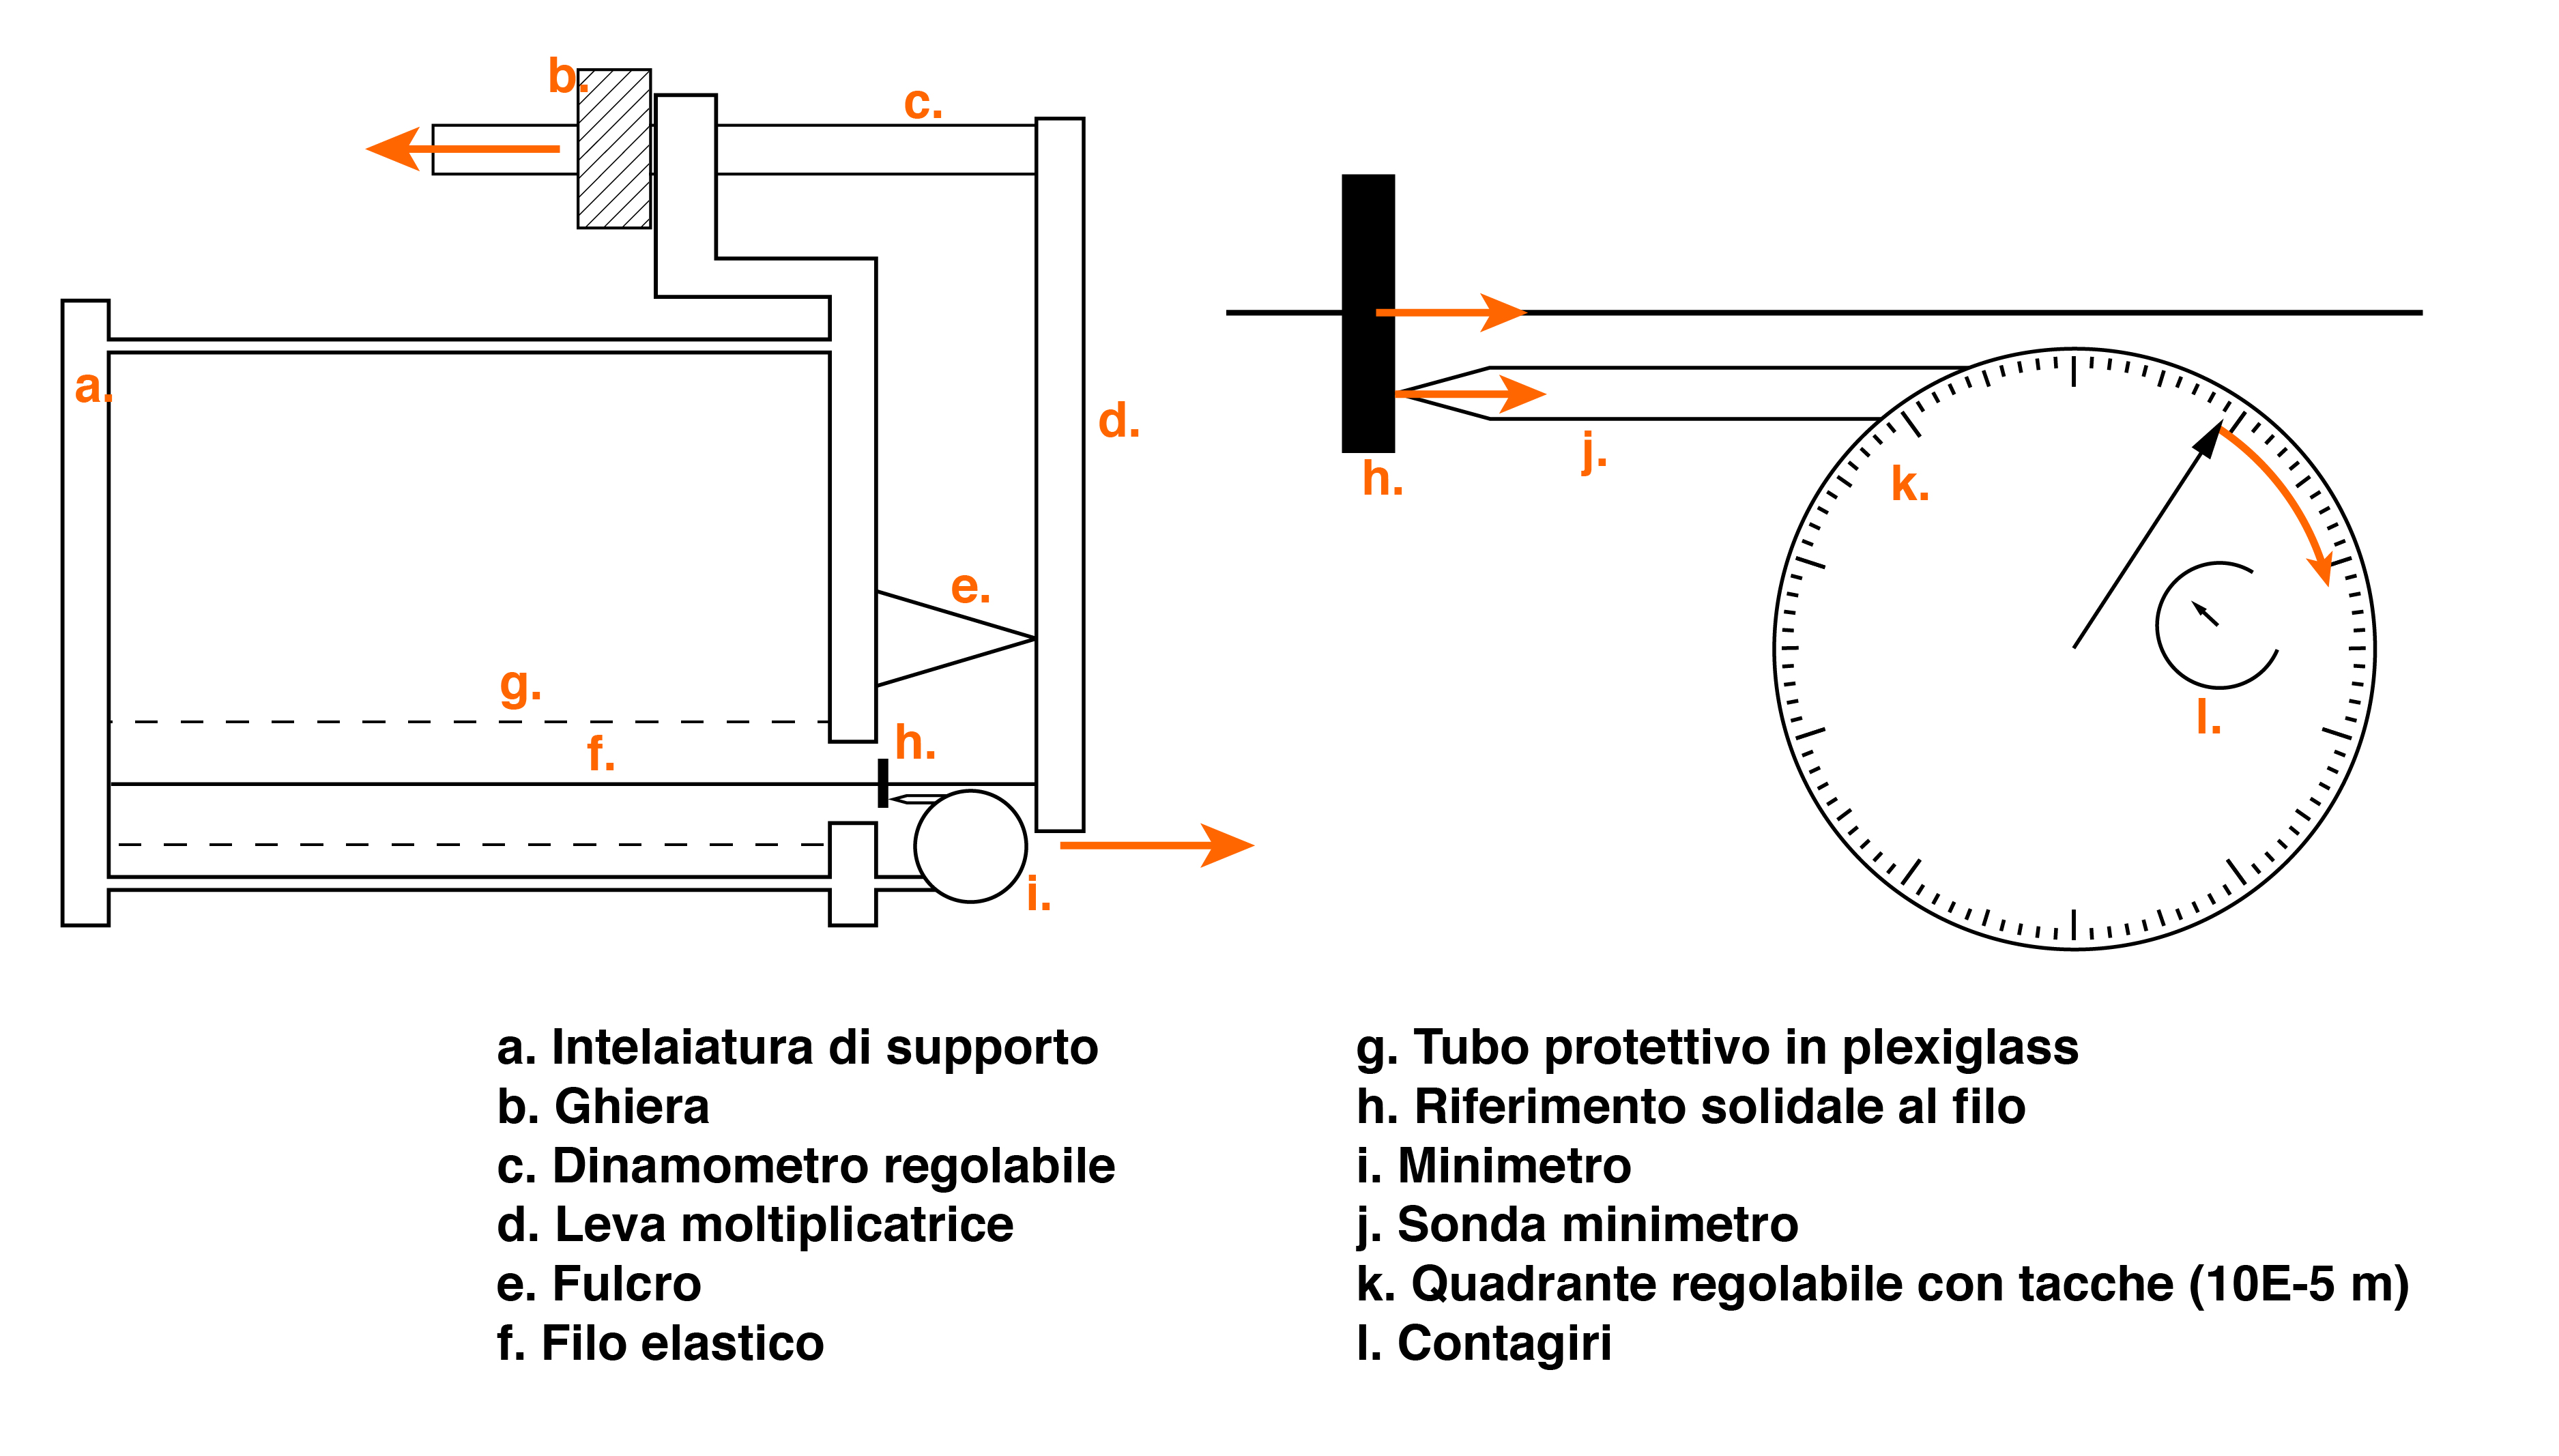
\includegraphics[width=12.5cm]{ApparatoSperimentale.jpg}
    \caption{Diagramma composizione apparato sperimentale}
    \label{fig:apparato_sperimentale}
\end{figure}
L'apparato sperimentale risulta così composto:
\begin{enumerate}
    \item Un cilindro metallico (acciaio, tungsteno o ottone) posto internamente ad un tubo protettivo a tutela di perturbazioni esterne. Lo stesso ha un'estremità fissata in maniera solidale alla struttura di supporto e nella parte finale presenta un disco forato, al fine di valutarne l'allungamento.
    \item Un minimetro a quadrante regolabile con sensibilità $S=\num{1e5} \si{m^{-1}}$ con sonda appoggiata al riferimento. E' presente inoltre un contatore interno al quadrante del minimetro che tiene conto dei giri completi compiuti dalla lancetta.
    \item Un dinamometro regolabile tramite una ghiera che, ruotando, varia la forza applicata al filo. L'unità di misura utilizzata è grammi peso, avente la più piccola tacca di lettura pari $\SI{100}{gp}$
    \item Una leva collegata al filo metallico e al dinamometro utilizzata per quadruplicare la forza esercitata dal dinamometro.
\end{enumerate}
Nel complesso sono stati impiegati 11 estensimetri diversi, dei quali vengono riassunte le caratteristiche nella Tabella \ref{tab:caratteristiche_estensimetri}.

\begin{table}
	\centering
	\begin{tabular}{lccc}
		    Materiale & \#& \multicolumn{1}{l}{Lunghezza}        & \multicolumn{1}{l}{Diametro}\\ 
		    &&$[\si{mm}] \pm\SI{2}{mm}$&$[\si{mm}] \pm\SI{1}{\percent}$\\
		\hline
\multirow{9}{*}{Acciaio} & {\cellcolor[rgb]{0.753,0.753,0.753}}1  & {\cellcolor[rgb]{0.753,0.753,0.753}}950  & {\cellcolor[rgb]{0.753,0.753,0.753}}0.33   \\
& 2 & 950 & 0.356  \\
& {\cellcolor[rgb]{0.753,0.753,0.753}}3  & {\cellcolor[rgb]{0.753,0.753,0.753}}950  & {\cellcolor[rgb]{0.753,0.753,0.753}}0.381  \\
& 4 & 950 & 0.305  \\ & {\cellcolor[rgb]{0.753,0.753,0.753}}5  & {\cellcolor[rgb]{0.753,0.753,0.753}}950  & {\cellcolor[rgb]{0.753,0.753,0.753}}0.3    \\
& 6 & 950 & 0.4                                        \\
& {\cellcolor[rgb]{0.753,0.753,0.753}}7  & {\cellcolor[rgb]{0.753,0.753,0.753}}950  & {\cellcolor[rgb]{0.753,0.753,0.753}}0.279  \\
& 8 & 600 & 0.279                                      \\
& {\cellcolor[rgb]{0.753,0.753,0.753}}9  & {\cellcolor[rgb]{0.753,0.753,0.753}}800  & {\cellcolor[rgb]{0.753,0.753,0.753}}0.279  \\
& 10 & 700 & 0.279                                      \\

Tungsteno & {\cellcolor[rgb]{0.753,0.753,0.753}}11 &{\cellcolor[rgb]{0.753,0.753,0.753}} 1000 &{\cellcolor[rgb]{0.753,0.753,0.753}} 0.25\\
Ottone                   & 12 & 1000 & 0.5   
\end{tabular}
	\caption{Estensimetri impiegati}
	\label{tab:caratteristiche_estensimetri}
\end{table}



\section{Metodi acquisizione dati}
Si specifica che i dati relativi alla prima parte sono stati trascritti da registrazioni video dell'apparato sperimentale composto dal decimo estensimetro. I dati invece impiegati nell'analisi sistematica dei vari estensimetri sono invece stati direttamente forniti in tabelle.\\
\begin{table}[h!]
    \centering
    \begin{tabular}{c|c|c|c|c|c|c}
        \toprule
        F_{letta} & \Delta x_{Operatore 1} & \Delta x_{Operatore 2} & \Delta x_{Operatore 3} & \Delta x_{Media} & Dev Std & Dev Std Media\\ 
         \si{[gpeso]}& [10^{-6}m] & [10^{-6}m] & [10^{-6}m] & [10^{-6}m] & [10^{-6}m]& [10^{-6}m]\\
        \midrule
        %\multirow{11}*{All}
       % &200&	-2&	-3&	-2&	-2,33333&	0,57735&	0,333333\\
        %&300&	223&	222&	225&	223,333&	1,52753&	0,881917\\
        %&400&	431&	431&	430&	430,667&	0,57735&	0,333333\\
        %&500&	660&	660&	660&	660&	0&	0\\
        %&600&	876&	878&	877&	877&	1&	0,57735\\
        %&700&	1093&	1091&	1092&	1092&	1&	0,57735\\
       % &800&	1310&	1311&	1310&	1310,33&	0,57735&	0,333333\\
        %&900&	1513&	1512&	1512&	1512,33&	0,57735&	0,333333\\
        %&1000&	1749&	1749&	1748&	1748,67&	0,57735&	0,333333\\
        %&1100&	1948&	1949&	1948&	1948,33&	0,57735&	0,333333\\
        %&1200&	2170&	2170&	2170&	2170&	0&	0\\
        \bottomrule
    \end{tabular}
    \caption{Dati Grezzi}
    \label{tab:dati_grezzi}
\end{table}
\begin{table}[]
\centering
\begin{tabular}{ll|l|l|l|l|l|l}
\hline
\multicolumn{2}{l}{F\_letta} & Delta\_x 1 & Delta\_x 2 & Delta\_x 3 & Delta\_x Media & Delta\_x Dev\_std & Dev\_std\_media \\
\multicolumn{2}{l}{gpeso} & {[}1e-6 m{]} & {[}1e-6 m{]} & {[}1e-6 m{]} & {[}1e-6 m{]} & {[}1e-6 m{]} & {[}1e-6 m{]} \\ \hline
Allungamento & 200 & -2 & -3 & -2 & -2,33333 & 0,57735 & 0,333333 \\
 & 300 & 223 & 222 & 225 & 223,333 & 1,52753 & 0,881917 \\
 & 400 & 431 & 431 & 430 & 430,667 & 0,57735 & 0,333333 \\
 & 500 & 660 & 660 & 660 & 660 & 0 & 0 \\
 & 600 & 876 & 878 & 877 & 877 & 1 & 0,57735 \\
 & 700 & 1093 & 1091 & 1092 & 1092 & 1 & 0,57735 \\
 & 800 & 1310 & 1311 & 1310 & 1310,33 & 0,57735 & 0,333333 \\
 & 900 & 1513 & 1512 & 1512 & 1512,33 & 0,57735 & 0,333333 \\
 & 1000 & 1749 & 1749 & 1748 & 1748,67 & 0,57735 & 0,333333 \\
 & 1100 & 1948 & 1949 & 1948 & 1948,33 & 0,57735 & 0,333333 \\
 & 1200 & 2170 & 2170 & 2170 & 2170 & 0 & 0 \\ \hline
Accorciamento & 1200 & 2170 & 2170 & 2170 & 2170 & 0 & 0 \\
 & 1100 & 1949 & 1950 & 1950 & 1949,67 & 0,57735 & 0,333333 \\
 & 1000 & 1727 & 1727 & 1727 & 1727 & 0 & 0 \\
 & 900 & 1514 & 1513 & 1514 & 1513,67 & 0,57735 & 0,333333 \\
 & 800 & 1303 & 1303 & 1305 & 1303,67 & 1,1547 & 0,666667 \\
 & 700 & 1082 & 1081 & 1082 & 1081,67 & 0,57735 & 0,333333 \\
 & 600 & 869 & 869 & 869 & 869 & 0 & 0 \\
 & 500 & 655 & 655 & 655 & 655 & 0 & 0 \\
 & 400 & 430 & 431 & 430 & 430,333 & 0,57735 & 0,333333 \\
 & 300 & 219 & 220 & 220 & 219,667 & 0,57735 & 0,333333 \\
 & 200 & 2 & 1 & 2 & 1,66667 & 0,57735 & 0,333333 \\ \hline
\end{tabular}
\caption{Dati Grezzi}
\label{tab:dati_grezzi}
\end{table}
Vengono qui esposti i due diversi metodi impiegati per raccogliere i dati nella prima parte.

\subsection{Primo metodo - Allungamento e Accorciamento}%aumento di 100 in 100
Come operazione preliminare si è agito sulla ghiera dell'estensimetro, manovrandola in modo tale che segnasse una tensione $F_{letta}=\SI{200}{gp}$ così da mettere in tensione il filo di metallo analizzato. Si è poi sollecitata delicatamente la manopola della sonda del minimetro così da eliminare l'eventuale contributo di giochi meccanici ed infine si è impostata la ghiera del minimetro in modo che lo zero del quadrante coincidesse con la posizione della lancetta maggiore. Dopo aver annotato il valore letto sul minimetro, tendendo in considerazione che una rotazione completa della lancetta corrisponde una variazione di lunghezza pari a $\num{1} \si{mm}$, si è manovrata la ghiera del dinamometro portandola alla tacca successiva, ovvero aumentando la forza letta di $\SI{100}{gp}$. Avendo cura di non oltrepassare la tacca e di smuovere la manopola della sonda di volta in volta, si sono annotati tutti i valori segnati dal minimetro. La ghiera è stata manovrata fino ad arrivare ad una forza letta di $\SI{1200}{gp}$. A tal punto si è diminuita la tensione esercitata dal dinamometro, variando sempre la $F_{letta}$ di $\SI{100}{gp}$, e annotando i valori del minimetro.\\

\subsection{Secondo metodo - Misure ripetute}%video 400 -1000
Riportato l'estensimetro con il dinamometro a $\SI{200}{gp}$ si sono eseguite misure ripetute. La procedura è consistita nel portare il dinamometro ad esercitare una tensione letta di $\SI{400}{gp}$, dapprima aumentandola a partire da $\SI{200}{gp}$, poi diminuendola a partire da $\SI{600}{gp}$. È stata prestata la massima attenzione nel non oltrepassare la tacca di $\SI{400}{gp}$. %Questa accortezza ha permesso di salvaguardare le misure da eventuali errori derivanti da fenomeni di isteresi meccanica.
Il procedimento è stato effettuato 18 volte in corrispondenza della tacca $\SI{400}{gp}$ per poi ripetere la presa dati in corrispondenza della tacca di $\SI{1000}{gp}$, variando in accorciamento fino a $\SI{800}{gp}$ e in allungamento fino a $\SI{1200}{gp}$.\\
E' opportuno precisare che l'analisi dei video è stata compiuta singolarmente: ogni operatore ha trascritto la lettura del minimetro corrispondente ad ogni misurazione, in modo da avere un campione più significativo e compiere una analisi statistica più accurata.

\section{Analisi dati}

\subsection{Prima parte - Verifica dell'elasticità meccanica e definizione miglior protocollo di misura}
Sono stati impiegati diversi metodi per il calcolo del coefficiente elastico del filo a seconda del metodo di raccolta dati.\\
Nella prima parte l'analisi si è svolta esclusivamente sull'estensimetro numero 10 riportato in Tabella \ref{tab:caratteristiche_estensimetri}. Nella seconda parte invece si è svolta un'analisi sistematica su tutti gli estensimetri in acciaio.

\subsubsection*{Primo Metodo - Misure in allungamento e accorciamento}
Per la prima acquisizione dati si è scelto di calcolare separatamente due diversi valori di K, mantenendo separati i dati raccolti quando il filo veniva allungato e quando il filo veniva accorciato. Si è utilizzato il metodo del minimo $\chi^2$ al fine di calcolare il coefficiente elastico, sfruttando la relazione lineare che lega l'allungamento o l'accorciamento del filo con la forza applicata per metterlo in tensione. La relazione è la seguente e prende il nome di legge di Hooke:
\begin{equation*}
       \left | x_i - x_0  \right |  = k \cdot  \left | \Delta F \right |
\end{equation*}
Partendo dai dati raccolti da ciascun operatore è stata calcolata la media delle acquisizioni relative alla stessa misurazione ed in seguito sono stati calcolati gli errori ad essa associati. Per il calcolo di quest'ultimo, al fine di non sottostimare l'errore si è  valutato opportunamente sia la deviazione standard della media e sia l' errore derivante dalla distribuzione uniforme, in modo da utilizzare la stima dell'errore più appropriata. Accadeva infatti che le misure dei tre operatori coincidessero e pertanto la $\overline{\sigma}$ fosse nulla. Per evitare un errore nullo si è tenuto in considerazione l'errore derivante dalla distribuzione uniforme con ptl pari a 10 micron e coefficiente di affidabilità pari a 10.
%ABBIAMO FORSE SOTTOSTIMATO L'ERRORE DUNQUE CAMBIARE QUESTA PARTE
Analogamente per l'incertezza sulla forza applicata si è usata la distribuzione triangolare considerando come ptl il doppio dello spessore della tacca incisa.
Per l'utilizzo del $\chi^2$ si sono confrontati i due errori e si è scelto strategicamente, in quando minore rispetto all'errore su $\Delta x$, di trascurare l'errore sulla forza e di utilizzarla come grandezza sull'asse delle ascisse.\\
Si sono ottenuti i valori dei coefficienti angolari K e delle intercette con l'asse delle ordinate per le misure in allungamento e in accorciamento ed è stato associato ad esse l'errore derivante dalla propagazione.\\
E' stata calcolata la compatibilità tra i due valori di K ottenuti e tra le due intercette. Si è fatto riferimento alle seguenti per valutare $\lambda$ e la sua bontà:
\begin{equation*}%Comp
    \label{eq:cases}
    \begin{cases}
    0<\lambda\leq 1, & \text{Ottima}\\
    1<\lambda\leq2, & \text{Discreta}\\
    2<\lambda\leq3, & \text{Pessima}\\
    3<\lambda, & \text{Non compatibile}\\
    \end{cases}
\end{equation*}
Successivamente gli errori sui coefficienti angolari e sulle intercette sono stati valutati nuovamente prendendo invece in considerazione la sigma a posteriori derivante dal chi quadro. Analogamente a quanto fatto precedentemente, si è calcolata nuovamente la compatibilità.\\
Viene riportato in Figura \ref{fig:GRAFICO ALL ACC} il grafico dell'andamento delle misure con le relative interpolazioni.
Per dare infine una stima del coefficiente K si è eseguita la media ponderata fra il $K_{all}$ e il $K_{acc}$ precedentemente ottenuti mediante la Formula \ref{equation:NOMEFORMULA PROPAGAZIONE}. Analogo procedimento è stato ripetuto per i valori delle intercette in allungamento ed in accorciamento. Vengono riportati in Tabella \ref{tab: TABELLA K E COMPATIBIITÀ}.

\subsubsection*{Secondo Metodo - Misure ripetute}
Per il calcolo di K tramite misure ripetute sono stati utilizzati due procedimenti differenti.\\
Nel primo caso, al fine di apprezzare eventuali evidenze sperimentali celate dal metodo precedente, si è optato per il calcolo del coefficiente di elasticità direttamente mediante la legge di Hooke, calcolando $\Delta x$ medi per ogni sottocampione di misurazioni.\\ 

In primo luogo si è proceduto con il calcolo delle medie delle misurazioni di ogni operatore, nello specifico per le misure di allungamento e accorciamento per $F_{letta}$ pari a $\SI{400}gp$ e $\SI{1000}gp$ distinguendo se si fosse raggiunta la tacca prescelta aumentando o diminuendo la forza dal dinamometro. Di ogni campione di lunghezze $\Delta x$, $F_{400, all}$, $F_{400, acc}$, $F_{10000, all}$ e $F_{10000, acc}$ si è calcolata la media, associandovi come errore la relativa $\sigma_{\overline{\Delta x}}$.\\
Per ogni campione, utilizzando la legge di Hooke, si sono ottenuti 4 valori differenti di coefficiente elastico ottenendo $K_{400, all}$, $K_{400, acc}$, $K_{1000, all}$ e $K_{1000, all}$ impiegando come $\Delta x$ quelli appena ricavati e come $\Delta F$ la differenza tra $\SI{400}{gp} / \SI{1000}{gp} - \SI{200}{gp}$ . L'errore di ogni K è stato calcolato utilizzando la propagazione degli errori tramite la seguente:
\begin{equation*}
\sigma_K \approx \sqrt{\left ( \frac{\partial K }{\partial F} \right )^2 \cdot \left ( \sigma_F \right )^2 + \left ( \frac{\partial K }{\partial \Delta_x} \right )^2 \cdot \left ( \sigma_{\Delta x} \right )^2 }
\end{equation*}

E' stata poi effettuata la media ponderata dei due coefficienti elastici "in allungamento" ($K_{400, all}$ e $K_{1000, all}$) e dei due "in accorciamento" ($K_{400, acc}$ e $K_{1000, acc}$) sempre associando il relativo errore. Infine per restituire un valore unico di K si è nuovamente calcolata la media ponderata fra questi due ultimi valori, associandovi l'errore. Infine si è valutata la compatibilità fra ${\langle K \rangle}_{all}$ e ${\langle K \rangle}_{acc}$. Tutti i dati citati sono riportati in Tabella \ref{tab: TABELLA DATI K SECONDO METODO con COMPATIBILITÀ}.\\

Il secondo metodo per le misure ripetute è consistito nel calcolo del $\chi^2$ su tutte le misure ottenute a 400gp e 10000gp con l'accortezza di distinguere i dati presi in allungamento ed in accorciamento. Operando secondo questo schema si sono ottenute due rette di interpolazione, una per i dati delle misure "in allungamento" ed una per quelli "in accorciamento". I due coefficienti angolari rappresentano i coefficienti rispettivamente di allungamento e di accorciamento e da essi si è ricavata la media ponderata, rappresentativa della costante elastica dell'estensimetro in esame e la compatibilità fra ${K}_{acc}$ e ${K}_{all}$. Vengono riportati i dati qui citati in Tabella \ref{tab: TABELLA SECONDO METODO SECONDA ACQUISIZIONE}

%MISURAZIONI DI 100 IN 100
% -CHI QUADRO
% ////-CAMPIONI DI K (NON SONO STATI FATTI)
%CONSECUTIVE
% -
%PROTOCOLLO DI MISURA
% - I GRAFICI CHE SERVON PER DIMOSTRARE POI< PARLANE E METTILI

\subsection{Seconda parte - Analisi sistematica degli estensimetri}
\subsubsection*{Stime di $K$}
Dai dati forniti, si sono calcolati i $\Delta x$ come differenza tra le misure $x_n$ e $x_0$ separatamente per allungamento e accorciamento, corrispondenti ad una $\Delta F_{app} =\left | F_{x, app} - F_{0, app} \right |$ e, conseguentemente, si sono valutati i $\Delta x$.
Similmente a quanto descritto nella prima acquisizione, dopo una rappresentazione grafica dei dati, si sono calcolati i $K_{all}$ e i $K_{acc}$ ed i relativi errori per tutti gli estensimetri dotati di filo in acciaio tramite il metodo del $\chi^2$
Per associare la giusta incertezza ai parametri del fit lineare si sono confrontati gli errori $\sigma_{\Delta x}$ e $\sigma_{\Delta x, posteriori}$, scegliendo tra queste l'errore che apportava il contributo maggiore, per evitare una possibile sottostima dell'errore sulle ordinate.
Si è poi calcolata la media ponderata tra i $K_{all}$ e $K_{acc}$ come stima del ${\langle K \rangle }\pm \sigma_{{\langle K\rangle }}$ e la compatibilità fra $K_{all}$ e $K_{acc}$ e fra $Intercetta_{all}$ e $Intercetta_{acc}$ per ciascun estensimetro come viene esposto nella Tabella \ref{tab: MEGA TABELLA CON TUTTI I K ALL E ACC DI TUTTI EST CON MEDI EPONDERATE E COMPATIBILIT}

\begin{figure}[H]
    \centering
    \subfloat[Estensimetro 1]{
        \label{fig:1_estensimetro}
        \includegraphics[width=7.5cm]{1_estensimetro.png}
    }
    \subfloat[Estensimetro 2]{
        \label{fig:2_estensimetro}
        \includegraphics[width=7.5cm]{2_estensimetro.png}
    }
    \newline
    \subfloat[Estensimetro 3]{
        \label{fig:3_estensimetro}
        \includegraphics[width=7.5cm]{3_estensimetro.png}
    }
    \subfloat[Estensimetro 4]{
        \label{fig:4_estensimetro}
        \includegraphics[width=7.5cm]{4_estensimetro.png}
    }
    \newline
    \subfloat[Estensimetro 5]{
        \label{fig:5_estensimetro}
        \includegraphics[width=7.5cm]{5_estensimetro.png}
    }
    \subfloat[Estensimetro 6]{
        \label{fig:6_estensimetro}
        \includegraphics[width=7.5cm]{6_estensimetro.png}
    }
    \newline
    \subfloat[Estensimetro 7]{
        \label{fig:7_estensimetro}
        \includegraphics[width=7.5cm]{7_estensimetro.png}
    }
    \subfloat[Estensimetro 8]{
        \label{fig:8_estensimetro}
        \includegraphics[width=7.5cm]{8_estensimetro.png}
    }
    
\end{figure}
\begin{figure}[h!]
    \centering
    \subfloat[Estensimetro 9]{
        \label{fig:9_estensimetro}
        \includegraphics[width=7.5cm]{9_estensimetro.png}
    }
\end{figure}

\newpage
\subsubsection*{Verifica della validità della legge di E}
Tramite l'analisi incrociata di diversi metodi è stata verificata la seguente legge utilizzata per il calcolo di E.
\begin{equation*}
    E=\frac{x_0}{S K}=\frac{4 x_0}{\pi D^{2}K}
    \label{equation:legge_e}
\end{equation*}
I metodi impiegati consistono nel verificare la proporzionalità dei parametri presenti nell'equazione sfruttandone la dipendenza lineare. Le varie verifiche della legge che sono state eseguite sono le seguenti:
\begin{enumerate}
    \item verificare la diretta proporzionalità tra K e la lunghezza di ogni estensimetro, $x_0$, di tutti gli estensimetri aventi stessa sezione $S$.
    \item verificare la diretta proporzionalità tra K e il rapporto della sezione $1/S$ di tutti gli estensimetri aventi stessa lunghezza a riposo $x_{0}$.
    \item calcolare il rapporto $R=\frac{K}{x_{0}}$, per tutti gli estensimetri con la stessa $S$, indipendentemente da $x_{0}$
    \item calcolare il prodotto $P= KD^2 $, per tutti gli estensimetri aventi la stessa $x_{0}$, indipendentemente da $S$
\end{enumerate}
Per la verifica della legge tramite il primo metodo si sono scelti i 4  estensimetri aventi la medesima sezione, e dunque lo stesso diametro, pari a 279. Tramite il calcolo dei K dei vari estensimetri selezionati, precedentemente effettuato, ed avendo a disposizione la lunghezza a riposo di ciascun filo, è stato elaborato un grafico avente sull'asse delle ascisse la lunghezza a riposo espressa in $mm$ e sull'asse delle ordinate il valore di K in $\micron$, associandone adeguatamente l'errore che era stato già calcolato nelle sezioni precedenti.

\begin{figure}[h!]
    \centering
    \subfloat[Verifica diretta proporzionalità tra K e $x_0$]{
        \label{fig:a_sezione_cost}
        \includegraphics[width=9cm]{a_sez_cost.png}
        }
\end{figure}
Per la verifica del secondo metodo (Grafico \ref{fig:a_lunghezza_cost}) sono stai selezionati invece gli estensimetri aventi lunghezza del filo d'acciaio pari a $\SI{950}{mm}$. E' stato realizzato un grafico avente sull'asse delle ascisse il valore di 1/S  calcolato per ogni estensimetro e sull'asse delle ordinate il valore di K dello stesso, associandone il relativo errore precedentemente calcolato.Si è inoltre calcolata una retta interpolante i dati rappresentata nel grafico con una retta tratteggiata di colore blu chiaro.\\
A causa dell'incongruenza tra il valore rappresentato in blu sul grafico e gli altri dati, si è deciso di eseguire una seconda analisi più accurata dei valori ottenuti, questa volta reiettando il dato considerato, e determinando una nuova retta interpolante,rappresentata in rosso nel grafico.
La reiezione è stata effettuata calcolando le probabilità di ottenere un dato valore in una regione ben delineata di grafico, ovvero tra la nuova retta interpolante e una parallela, ottenuta aumentando l'intercetta dell' interpolante di un valore arbitrariamente scelto. Anche tenendo conto dell'errore del quale risulta affetto il dato reiettato, si è riscontrato che la probabilità di riottenere lo stesso è molto inferiore rispetto a quella calcolata degli altri dati.
%bisogna specificare nella discussione tutto quello che è stato fatto, occhio alla distinzione tra analisi e discusisione 


\begin{figure}[h!]
    \centering
    \subfloat[Verifica diretta proporzionalità tra K e 1/S]{
        \label{fig:a_lunghezza_cost}
        \includegraphics[width=9cm]{a_lung_cost .png}
        }
\end{figure}



Per quanto riguarda il calcolo del rapporto R, come per i metodi precedenti, si sono selezionati solo alcuni estensimetri,ovvero quelli aventi la stessa sezione ed è stato eseguito il calcolo per ognuno di essi del rapporto R tramite la seguente formula: $R=\frac{K}{x_{0}}$. Ad esso è stato associato un errore calcolato tramite la propagazione degli errori, ovvero 
\begin{equation*}
    \sigma_R \approx \sqrt{\left ( \frac{\partial R }{\partial K} \right )^2 \cdot \left ( \sigma_K \right )^2 + \left ( \frac{\partial R }{\partial x_0} \right )^2 \cdot \left ( \sigma_{x_0} \right )^2 }
\end{equation*}

In seguito è stato generato un grafico contenete i valori calcolati, nello specifico sull'asse delle ascisse sono stati posizionati i valori delle lunghezze a riposo degli estensimetri presi in considerazione e sull'asse delle ordinate il valore di R calcolato. E' stata poi determinata una retta interpolante i 3 dati rappresentati sul grafico.


\begin{figure}[h!]
    \centering
    \subfloat[Verifica del rapporto R]{
        \label{fig:a_lunghezza_cost}
        \includegraphics[width=9cm]{rapporto.png}
        }
\end{figure}
Infine per il quarto metodo, consistente nel calcolo del prodotto P, sono stati selezionati gli estensimetri aventi la stessa lunghezza a riposo ed è stato calcolato per ognuno di essi il quadrato del diametro. Conseguentemente è stato ricavato P tramite la seguente : $P= K \cdot D^2 $, e ad esso è stato attribuito l'errore  ricavato dalla propagazione degli errori, ovvero 

\begin{equation*}
    \sigma_P \approx \sqrt{\left ( \frac{\partial P }{\partial K} \right )^2 \cdot \left ( \sigma_K \right )^2 + \left ( \frac{\partial R }{\partial D} \right )^2 \cdot \left ( \sigma_D \right )^2 }
\end{equation*}
E' stata conseguentemente determinata una retta interpolante le coppie di dati ed è stata rappresentata nel grafico in blu tratteggiato.\\
In quanto si dubitava della veridicità del dato rappresentato in blu nel grafico, così come già eseguito per la diretta proporzionalità tra K e 1/S, tramite il medesimo ragionamento è stata eseguita la reiezione di quest'ultimo ed è stata determinata una nuova retta interpolante i dati ottenuti, rappresentata in rosso nel grafico sottostante.

\begin{figure}[h!]
    \centering
    \subfloat[Verifica del prodotto P]{
        \label{fig:a_lunghezza_cost}
        \includegraphics[width=9cm]{prodotto.png}
        }
\end{figure}

\subsubsection*{Stime di $E$}
Per la stima del modulo di Young sono stati impiegati e confrontati 3 metodi differenti.

\paragraph{Primo Metodo} Nel primo metodo si è calcolato E come media ponderata di $E_{all}$ e $E_{acc}$ calcolati singolarmente tramite la legge \ref{equation:legge_e}. Gli errori associati a $E_{all}$ e $E_{acc}$ sono stati ottenuti dalla seguente equazione:
\begin{equation*}
    \sigma_{E} = E\sqrt{\left(\frac{\sigma_{x_{0}}}{x_{0}}\right)^2+\left(\frac{\sigma_{K}}{K}\right)^2+4\left(\frac{\sigma_{D}}{D}\right)^2}
    \label{eq:propagazione_particolare}
\end{equation*}
L'errore associato alla E invece è stato calcolato come errore della media ponderata (equazione \ref{eq:errore_media_pond}).

\paragraph{Secondo Metodo} Inversamente a quanto fatto precedentemente, nel secondo metodo è stato calcolato K come media ponderata di $K_{all}$ e $K_{acc}$ e a partire da esso è stato ricavato E e l'errore $\sigma_{E}$ grazie rispettivamente alle relazioni \ref{equation:legge_e} e \ref{eq:propagazione_particolare}

\paragraph{Terzo Metodo} Nell'ultimo metodo si è deciso di utilizzare campioni di $K_{all}$ e $K_{acc}$ ottenuti a partire da $\Delta x$  non consecutivi e statisticamente indipendenti come 
\begin{equation*}
    \biggl\{ K_{all} = \frac{|\Delta x_{all}|}{|\Delta F_{app}|}\biggr\}_{all}
    \hspace{1cm} e \hspace{1cm}
    \biggl\{ K_{acc} = \frac{|\Delta x_{acc}|}{|\Delta F_{app}|}\biggr\}_{acc}
\end{equation*}
Gli errori associati sono stati calcolati tramite propagazione. Per far ciò è stato necessario inoltre calcolare $\sigma F$ dalla distribuzione uniforme ponendo come più piccola tacca di misura $\approx \SI{0.1}{N}$ e coefficiente di affidabilità 1. Successivamente si sono calcolate separatamente $E_{all}$ e $E_{acc}$ con i relativi errori come fatto per il metodo 2 e facendone la media ponderata si è ottenuta la stima di E.

%Compatibilità tra le E?

\newpage

\section{Discussione dei risultati}
% - ERRORE DI DESALVADOR

\subsection{Prima parte}
\subsubsection*{Primo metodo misurazione}
Sin da una prima analisi sui dati degli operatori risulta che la $\sigma_{\overline{x}}$ risulta nulla in quanto misure tra loro identiche. Non essendo ciò fisicamente possibile, per non sottostimare l'errore si è impiegata la sigma derivante dalle distribuzione uniforme. I parametri ad essa associati risultano ptl di 10 micron, in quanto ogni tacca incisa rappresenta 10 micrometri ed un coefficiente di affidabilità pari a 10. Questa scelta è motivata dal fatto che è possibile riconoscere posizioni della lancetta del minimetro tra due tacche incise fino a poter stimare la variazione di un singolo micron. Si è optato per la distribuzione uniforme al posto di quella triangolare in quanto rappresenta più difficilmente una sottostima dell'errore.
Va specificato che un analogo confronto è stato compiuto per tutte le $\sigma_{\overline{x}}$. Come accennato talora la sigma sulla misura fosse inferiore alla sigma uniforme, essa veniva sostituita sempre per non sottostimare l'errore. Per l'incertezza su $\Delta F$ si è scelto arbitrariamente come ptl il doppio dello spessore della tacca incisa in quanto si è assunto come errore massimo possibile dovuto ad un eventuale disallineamento dell'operatore.\\
Nella realizzazione del grafico, a ciascuna misura $\Delta x$ è stata attribuita come incertezza la propagazione degli errori delle due misure con cui si è compiuta la differenza. Poiché questi ultimi risultavano essere sempre pari alla sigma della distribuzione triangolare, ogni $\Delta x$ aveva ugual peso nell'interpolazione tramite chi quadro.\\
Ottenuti i parametri del chi quadro sull'allungamento e sull'accorciamento con le sigma y precedentemente ottenute, si sono rieseguiti i calcoli utilizzando la sigma a posteriori. Sin da una prima analisi sigma a posteriori è di circa un ordine di grandezza più grande rispetto a sigma y. Questo controllo pur avendo aumentato l'errore casuale sui parametri del fit ha permesso di ottenere delle stime più attendibili e verisimili. Le compatibilità fra parametri in allungamento ed in accorciamento con la sigma y risultano incompatibili sia per il coefficiente angolare sia per l'intercetta, mentre con la sigma a posteriori risultano ottime. Questo comportamento è dovuto ad un valore molto piccolo nell'errore casuale, tale da generare valori molto alti nella formula della compatibilità, facendone perdere significato in relazione al fenomeno osservato.Si è assunto di utilizzare la sigma a posteriori come incertezza per il computo degli errori nei parametri in ogni caso in cui essa fosse maggiore delle singole incertezze delle misure in ordinata.\\
Il confronto fra i coefficienti angolari mette in evidenza il comportamento elastico del filo. La compatibilità ottima infatti conferma un comportamento pressoché identico nelle fasi di accorciamento e di allungamento. Va però osservato che in allungamento il coefficiente elastico, pari al coefficiente angolare, risulta leggermente maggiore. Si ipotizza che questo risultato sia dovuto al processo di allungamento e accorciamento stesso, ovvero che il materiale si comporti in maniera leggermente diversa a seconda del procedimento meccanico a cui è sottoposto.
Il confronto fra le intercette, pur generando tra loro valori compatibili indicherebbe la presenza di un allungamento anche in assenza di forze applicate. Questo comportamento è ricondotto ad un errore di natura sconosciuta, probabilmente dovuto ad un errore sistematico. Ci si aspetta infatti che l'intercetta corrisponda all'origine degli assi. Tuttavia si evidenza che la compatibilità dell'intercetta con l'origine degli assi ($0\pm \sigma_{\Delta x, pos}$) è ottima ($\approx \num{0.5}$) e dunque un errore trascurabile.

\subsubsection*{Secondo metodo misurazione}
La possibilità di compiere misure ripetute mette in marcata evidenza la differenza che intercorre tra le misurazioni in allungamento e in accorciamento. I Grafici \ref{fig:GRAFICO ISTERESI1 e GRAFICO ISTERESI 2} infatti evidenziano sia le dispersioni dovute alle diverse letture degli operatori e alla distribuzione uniforme, analogamente a quanto discusso per l'acquisizione precedente, sia la tendenza delle misure prese in allungamento ad essere maggiori di quelle prese in accorciamento, per $F_{400}$ e per $F_{1000}$.
Appare inoltre che aumentando il numero consecutivo della misurazione ci sia un lieve aumento della lunghezza misurata sul minimetro, come evidenziato dalle rette a coefficiente angolare positivo del fit. Si ipotizza pertanto che un ripetuto allungamento e accorciamento del filo vada ad alterarne il comportamento. 
Si osserva tuttavia un'eccezione alla retta in \ref{fig: QUELLA DEL 400} relativa alle misure in accorciamento. La pendenza negativa è probabilmente attribuibile alle ultime tre misure, da considerare forse affette da errore sistematico subentrato solo in questi ultimi tre casi. Quanto affermato trova fondamento nella specularità degli andamenti delle misure in allungamento e accorciamento, comportamento forse attribuibile ad un processo di isteresi meccanica.\\
A seguito di queste considerazioni si sono assunti come valori rappresentativi dei campioni di misure in allungamento e accorciamento, sia a 400 che a 1000, la media e la deviazione sulla media degli stessi.
Questi valori sono stati poi impiegati per il calcolo dei K. Si noti che si sono tenute separate le misure eseguite in allungamento e accorciamento il più possibile, fino a quando non si è eseguita la media ponderata  fra $K_{acc}$ e $K_{all}$. Questa accortezza è il risultato di una scelta arbitraria compiuta a priori nel processo di analisi dati, in modo da risultare coerente con l'obiettivo di mostrare una possibile componente di errore sistematico.%AGGGIUNGERE ERRORE SISTEMATICO DE SALAVDOR


\subsection{Seconda parte}

\section{Margini di miglioramento}

\section{Conclusione}

\section{Appendice}

\subsection{Formulario}
\textbf{Media, deviazione standard, deviazione standard della media}
\begin{align*}
   % \begin{aligned}
        \overline{x}&=\sum\limits_{i=1}^{N} \frac{x_{i}}{N}&
        \sigma&=\sqrt{\frac{\sum\limits_{i=1}^{N} (x_{i}-\overline{x})}{N-1}}&
        \sigma_{\overline{x}}&=\frac{\sigma}{\sqrt{N}}
   % \end{aligned}
\end{align*}\\

\textbf{Media Ponderata}
\begin{equation*}\
    x_i=\frac{\sum_{i=1}^{N}\frac{x_i}{\sigma_{x_i}}}{\sum_{i=1}^{N}\frac{1}{\sigma_{x_i}}} \label{eq:media_ponderata}
\end{equation*}

\textbf{Errore Media Ponderata}
\begin{equation*}
     \sigma_{x_i}=\sqrt{\frac{1}{\sum_{i=1}^{N}\frac{1}{\sigma_{i}^{2}}}}\label{eq:errore_media_pond}
\end{equation*}

\textbf{Formule per il ${\chi}^2$}
\begin{equation*}
        \begin{cases}
    a=&\frac{1}{\Delta}[(\sum\limits_{i=1}^{N}{x_{i}^{2}})\cdot(\sum\limits_{i=1}^{N}{y_{i}})-(\sum\limits_{i=1}^{N}{x_{i}})\cdot(\sum\limits_{i=1}^{N}{x_{i}y_{i}})] \\ 
    b=&\frac{1}{\Delta }\cdot \left [N\cdot \left ( \sum\limits_{i=1}^{N}x_i y_i \right )-\left ( \sum\limits_{i=1}^{N}x_i \right )\cdot \left ( \sum\limits_{i=1}^{N}y_i \right )  \right ]\\
    \Delta=& N\cdot \sum\limits_{i=1}^{N} x_i^{2} - \left ( \sum\limits_{i=1}^{N}x_i \right )^{2}\\
    \end{cases}
\end{equation*}
\begin{equation*}
    \begin{cases}
    \sigma_{a}=&\sigma_{y}\cdot\sqrt{\frac{\sum_{i=1}^{N}{x_{i}^{2}}}{\Delta}} \\
    \sigma_{b}=&\sigma_y\cdot \sqrt{\frac{N}{\Delta }}\\
    \end{cases}
    \label{equation:err_chi_quadro}
\end{equation*}
\\
\textbf{Formula di propagazione degli errori casuali}\\

Sia z=($x_1$,...;$x_N$) funzione di N variabili casuali $x_1$,...,$x_N$ e sia ${x_i^\ast}$=($x_1^\ast$,...,$x_N^{\ast}$) l'insieme di tutti i valori veri associati a tali variabili, si ha 

\begin{equation*}
    \sigma_z^{2}\approx  \sum_{i=j=1}^{N}\left ( \frac{\partial z}{\partial x_i}\Big|_{x_i^{\ast}} \right )^{2}\cdot\sigma_{x_i}^{2} +\sum_{i=1,j=1,i\neq j}^{N}\left (\frac{\partial z }{\partial x_i}\Big|_{x_i^{\ast}} \right ) \cdot \left ( \frac{\partial z}{\partial x_j} \Big|_{x_j^{\ast}} \right )\cdot cov(x_i,x_j)\label{eq:prop_errori}
\end{equation*}
E' stato utilizzato il simbolo $\approx$ in quanto si è scelto di troncare al primo termine lo sviluppo in serie di Taylor.\\


\textbf{Formula calcolo compatibilità}\\
\begin{equation*}
    \lambda=\frac{\left|a-b\right|}{\sqrt{\sigma^{2}_{a}+\sigma^{2}_{b}}}
\end{equation*}\\

\subsection{Codice sorgente}

\end{document}*
